\subsubsection{Kettenmatrix}\label{subsubsec:kettenmatrix}

Die Kettenmatrix ist eine Variante, um das Verhalten von 2-Toren zu beschreiben. Andere Varianten sind die Z-Matrix oder die Y-Matrix. Die Kettenmatrix hat jedoch den Vorteil, dass man in Serie geschaltene 2-Tore ohne grossen Aufwand zusammen rechnen kann. Sobald man die einzelnen Kettenmatrizen gebildet hat und die Schaltung soweit vereinfacht ist, dass nur noch in Serie geschaltene Ketten-Matrizen vorzufinden sind, können diese miteinander multipliziert werden. Das Matrix-Produkt stellt dann die Kettenmatrix der Gesamtschaltung dar. Folgenden gängigen Schaltungen helfen, die Kettenmatrizen der einzelnen Schaltungsteilen zu bilden (siehe Anhang: 2-Tor Tabellen). \textcolor{red}{\textbf{TODO:Quelle ganzes kapitel}}

Die Längsimpedanz lässt sich anhand der Kettenmatrix A\textsubscript{L} (Formel \ref{equ:horizImpedance}) darstellen
\begin{figure}[H]
	\begin{minipage}[h]{0.45\linewidth}
		\centering
		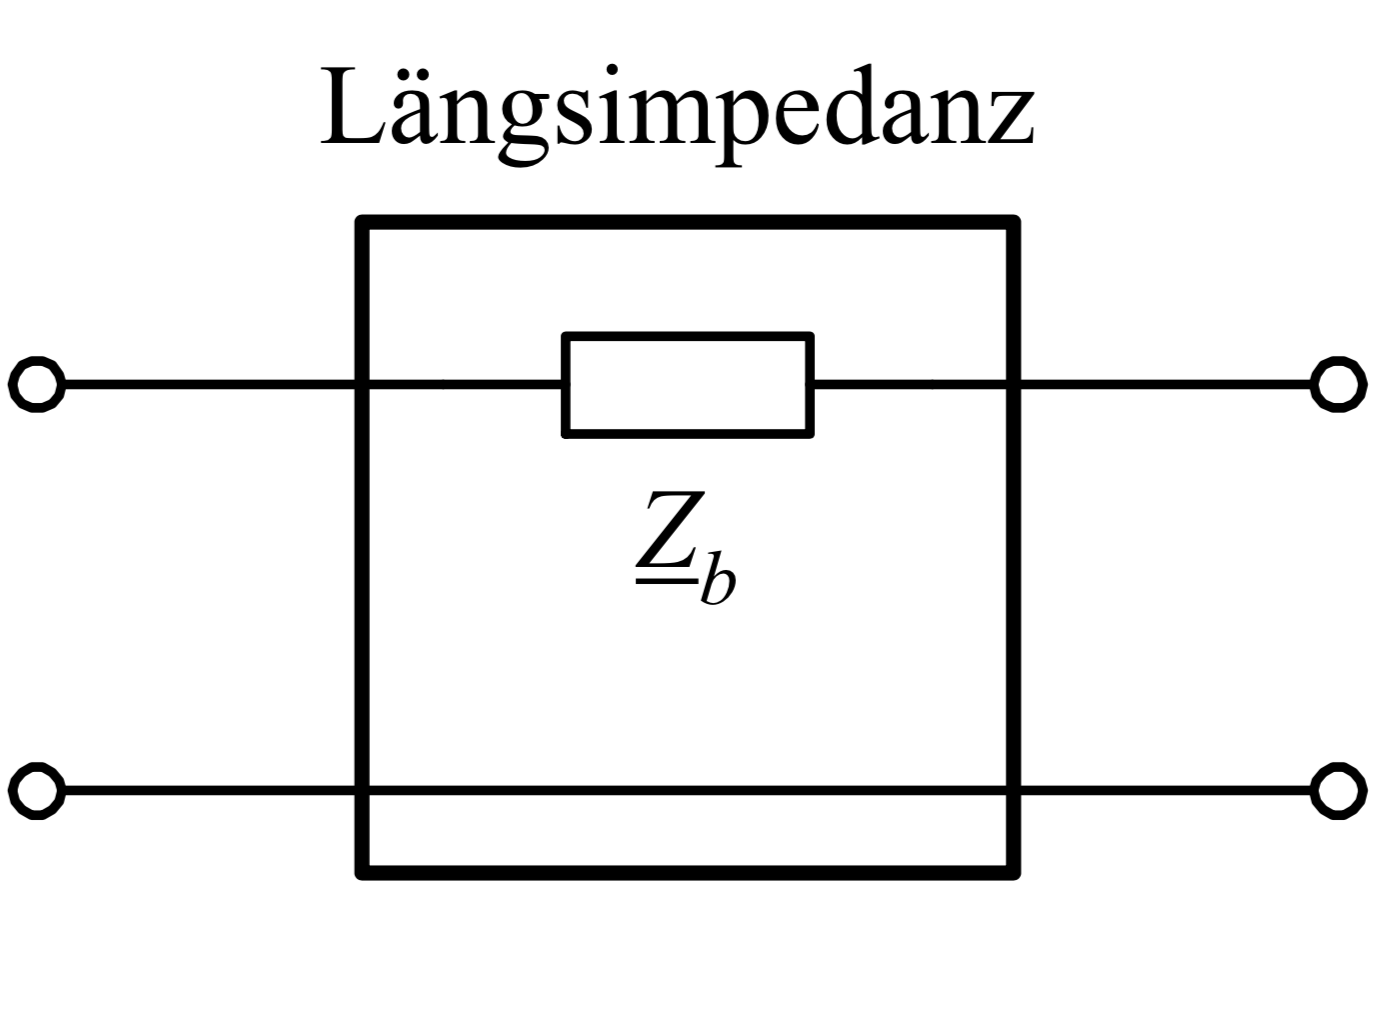
\includegraphics[width = 3cm]{h_impedance.png}
		\caption{Längsimpedanz}
	\end{minipage}
	\begin{minipage}[h]{0.45\linewidth}
		\centering
		\begin{equation}\label{equ:horizImpedance}
			A_L = \left[\begin{matrix}
			1&\underline{Z}_b\\0&1
			\end{matrix}\right]
		\end{equation}
	\end{minipage}
\end{figure}

Die Querimpedanz lässt sich anhand der Kettenmatrix A\textsubscript{Q} (Formel \ref{equ:verticImpedance}) darstellen

\begin{figure}[H]
	\begin{minipage}[h]{0.45\linewidth}
		\centering
		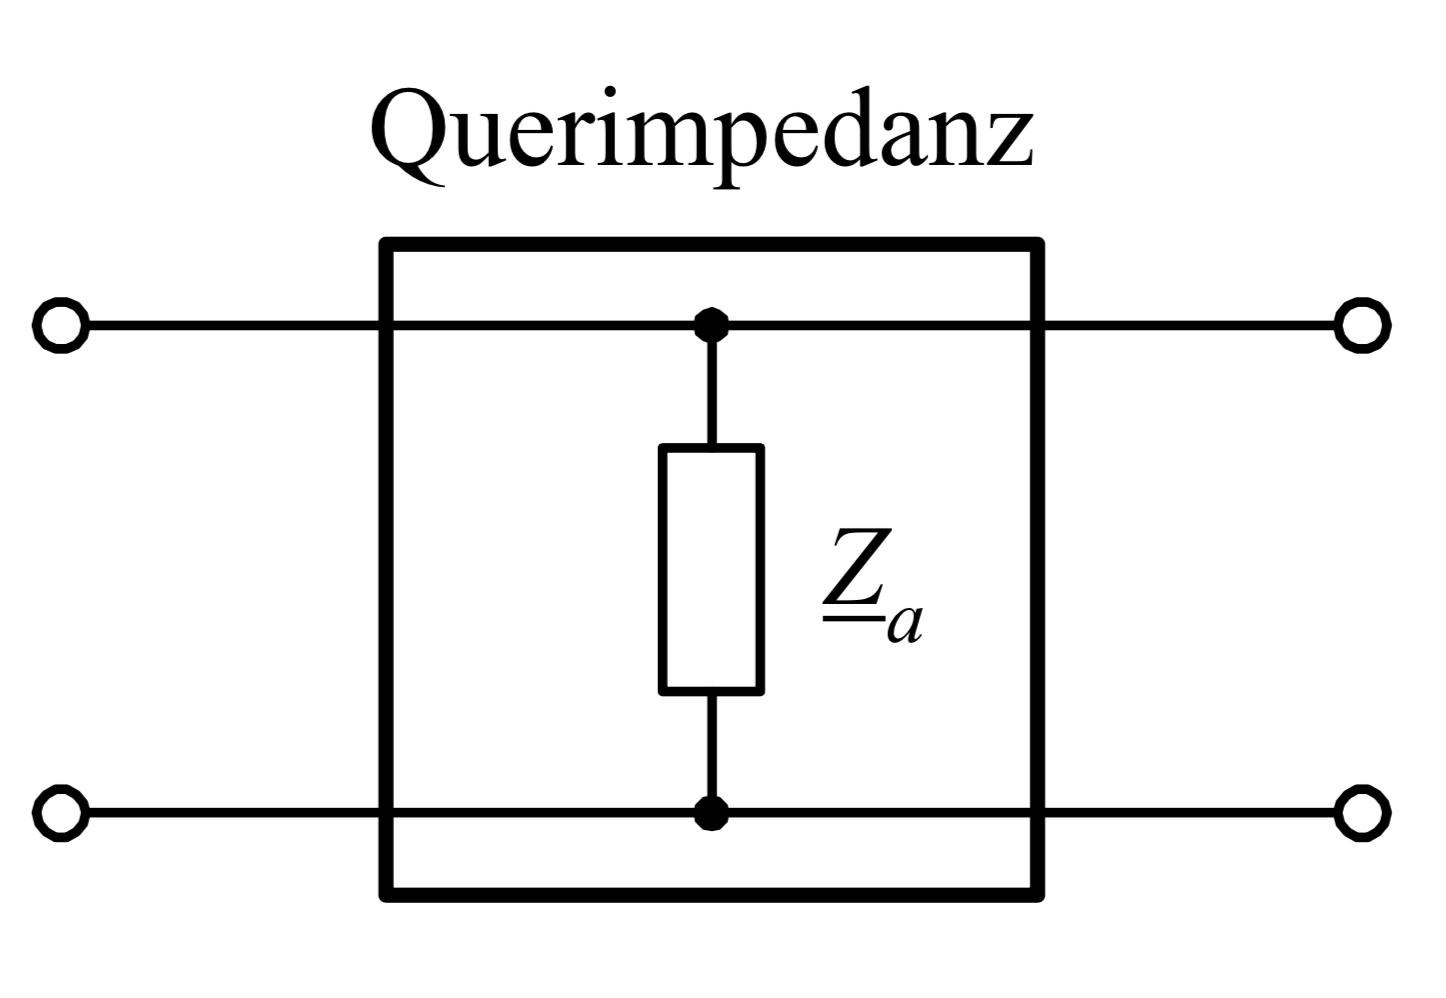
\includegraphics[width = 3cm]{v_impedance.png}
		\caption{Querimpedanz}
	\end{minipage}
	\begin{minipage}[h]{0.45\linewidth}
		\centering
		\begin{equation}\label{equ:verticImpedance}
			A_Q = \left[\begin{matrix}
			1&0\\\frac{1}{\underline{Z}_a}&1
			\end{matrix}\right]
		\end{equation}
	\end{minipage}
\end{figure}

\textcolor{red}{\textbf{TODO:Quelle Bilder}}

Sobald die Kettenmatrix einer Schaltung gebildet wurde, kann diese direkt in die Streuparameter umgewandelt werden. Der $s_{21}$ Parameter kann wie in Formel \ref{equ:s21} beschrieben, durch Einsetzten der Kettenmatrix bestimmt werden. Für den Widerstand $R_w$ muss die verwendete Bezugsimpedanz eingesetzt werden.
\begin{equation}\label{equ:s21}
s_{21} = \frac{2}{A_{11}+\frac{A{12}}{R_w}+A_{21}*R_w+A_{22}}
\end{equation}
Die Indexierung der Kettenmatrix wird in der Formel \ref{equ:A_index} gezeigt.
\begin{equation}\label{equ:A_index}
	A = \left[\begin{matrix}
	A_{11}&A_{12}\\A_{21}&A_{22}
	\end{matrix}\right]
\end{equation}
\newpage

